\vspace{-0.7\baselineskip}
\section{Experiments}
\label{sec:experiments}
\vspace{-0.3\baselineskip}

In this section, we introduce implementation details, datasets, evaluation metrics. An ablation study of how much each component of the framework contributes and a performance comparison with other supervised or unsupervised methods are also presented.

\vspace{-0.3\baselineskip}
\subsection{Implementation details.}
\vspace{-0.1\baselineskip}
Our framework is implemented with publicly available TensorfFlow \cite{abadi2016tensorflow} platform and has 34 million trainable variables in total. During training, Adam optimizer is applied with parameters $\beta_1 = 0.9$, $\beta_2=0.000$, $\epsilon=10^{-8}$. Learning rate and batch size are set to be $2\times10^{-3}$ and $4$ respectively. Batch normalization \cite{ioffe2015batch} is not used as we didn't observe a performance improvement with it. Following \cite{zhou2017unsupervised}, we use the same loss balancing for $\lambda_s, \lambda_m$, and correct the depth by a scale factor. We set $\lambda_n=1$ and $\lambda_g=\lambda_s$. %That is, multiplying the predicted depth by a factor $\hat{f}$: $\hat{f} = \mathrm{median}(D_{gt}) / \mathrm{median}(D_{pred})$. As the predicted depths are not absolute depth but defined up to a scale, 

The length of input sequence is fixed to be 3 and the input frames are resized to $128 \times 416$. The middle frame is treated as the target image and the other two are source images. With the settings above, the network starts to show meaningful results after 3 epochs, and converges at the end of the 5th epoch. With a Nvidia Titan X (Pascal), the training process takes around 6 hours. The number of epochs and absolute time needed is much less than \cite{godard2016unsupervised} (50 epochs, 25 hours) and \cite{zhou2017unsupervised} (15 epochs).


\begin{table*}[t]
\centering
\caption{Depth performance of our framework variants on the KITTI split.}
\label{tbl:ablation}
\fontsize{8}{9}\selectfont
\bgroup
\def\arraystretch{1.2}
\begin{tabular}{c|c|c|c|c|c|c|c}
\thickhline
\multirow{2}{*}{Methods}  & \multicolumn{4}{c|}{Lower the better} & \multicolumn{3}{c}{Higher the better}                  \\ \cline{2-8} 
                          & Abs Rel  & Sq Rel  & RMSE  & RMSE log & $\delta < 1.25$ & $\delta < 1.25^2$ & $\delta < 1.25^3$ \\ \hline
Ours (no d-n)             & 0.208    & 2.286   & 7.462 & 0.297    & 0.693           & 0.875             & 0.948             \\
Ours (smooth no gradient) & 0.189    & 1.627   & 7.017 & 0.280    & 0.713           & 0.891             & 0.957             \\
Ours (no img grad for d-n)    & 0.179    & 1.566   & 7.247 & 0.272    & 0.720           & 0.895             & 0.959             \\
Ours (no normal smooth)   & 0.172    & 1.559   & 6.794 & 0.252    & 0.744           & 0.910             & 0.969             \\ \hline
\end{tabular}
\egroup
\vspace{-0.7\baselineskip}
\end{table*}

\vspace{-0.5\baselineskip}
\subsection{Datasets and metrics}
\vspace{-0.3\baselineskip}
\textbf{Training.}
Theorectically, our framework can be trained on any frame sequences captured with a monocular camera. To better compare with other methods, we evaluate on the popular KITTI 2015 \cite{geiger2012we} dataset. It is a large dataset suite for multiple tasks, including optical flow, 3D object detection, tracking, and road segmenations, \etc The raw data contains RGB and gray-scale videos, which are captured by stereo cameras from 61 scenes, with a typical image size of $1242 \times 375$.

In our experiments, videos captured by both left and right cameras are used for training, but treated independently. We follow the same training sequences as \cite{zhou2017unsupervised,eigen2014depth}, excluding frames from test scenes and static sequences. This results in 40,109 trainig sequences and 4431 validation sequences. Different from \cite{godard2016unsupervised}, no data augmentation has been performed.

\textbf{Testing.}
There are two sets of KITTI 2015 test data: (1) Eigen split contains 697 test images proposed by \cite{eigen2014depth}; (2) KITTI split contains 200 high-quality disparity images provided as part of official KITTI training set.  To better compare with other unsupervised and supervised methods, we present evaluation methods on both two splits. 

The depth ground truth of Eigen split is generated by projecting 3D points scanned from Velodyne laser to the camera view. This produces depth values for less than 5\% of all pixels in the RGB images. To be consistent when comparing with other methods, the same crop as in \cite{eigen2014depth} is performed when testing. The depth ground truth of KITTI split contains sparse depth map with CAD models in place of moving cars. It provides better quality depth than projected Velodyne laser scanned points but has ambiguous depth value on object boundaries where the CAD model doesn't align with the images. The predicted depth is capped at 80 meters as in \cite{godard2016unsupervised} and \cite{zhou2017unsupervised}.

The normal ground truth for two splits is generated by applying our depth-to-normal layer on inpainted depth ground truth, where the same inpainting algorithm as \cite{silberman2012indoor} is used. For both depth and normal, following \cite{eigen2014depth}, only the pixels with laser ground truth are used.

\textbf{Metrics.} We apply the same depth evaluation and normal evaluation metrics as in \cite{eigen2015predicting}. For depth evaluation, we use the code provided by~\cite{zhou2017unsupervised} and for normal, we implement ourselves and verified the correctness through validating normal results of \cite{eigen2015predicting} over the NYUv2 dataset.

% Abs Rel: $\frac{1}{|D|}\sum_{d_{pred}\in D}|d_gt - d_{pred}|/d_gt$

% Sq Rel: $\frac{1}{|D|}\sum_{d_{pred}\in D}||d_gt - d_{pred}||^2/d_gt$

% RMSE: $\sqrt{\frac{1}{|D|}\sum_{d_{pred}\in D}||d_{gt} - d_{pred}||^2}$

% RMSE log: $\sqrt{\frac{1}{|D|}\sum_{d_{pred}\in D}||\log d_{gt} - \log d_{pred}||^2}$

% $\delta<thr$: $\%$ of $d_{pred}\in D$, s.t. $max(\frac{d_gt}{d_{pred}}, \frac{d_{pred}}{d_{gt}})<thr$

% mean: $\frac{1}{|N|}\sum_{n_{pred}\in N}(n_{gt}\cdot n_{pred})$

% median: $median([(n_{gt}\cdot n_{pred})]_{n_{pred} \in N})$

% degree: $\%$ of $n_{pred} \in N$, s.t. $(n_{gt}\cdot n_{pred}) < degree$


\vspace{-0.6\baselineskip}
\subsection{Ablation study}
\vspace{-0.3\baselineskip}
To investigate different components proposed in \secref{sec:approach}, we perform an ablation study by removing each one from our full model and evaluating on the KITTI split.

\textbf{Depth-normal consistency.} By removing normal-to-depth layer (\equref{eq:depth}), the inverse warping process (Sec. \ref{chap:warping}) takes an image and directly predicted depth map from the input. We show the performance at the row ``Ours (no d-n)" in Tab. \ref{tbl:ablation}. It is much worse than our full model on Kitti shown in Tab. \ref{tbl:sota}.
Notice that with depth-normal consistency, the network not only performs better but converges faster. In fact, our full model converges after 5 epochs, while the network without such consistency converges at 15th epoch.

% We explore the effectivness of adding image gradient into smoothness term.
\textbf{Image gradient in smoothness term.} To validate image gradient for depth and normal smoothness in \equref{eqn:regular}, 
we setting $\alpha=0$. The results is shown as ``Ours (smooth no gradient)" in Tab. \ref{tbl:ablation}. It makes less impoact than depth-normal consistency, but still helps the performance.

\textbf{Image gradient in normal-depth consistency.} We set $\omega=1$ in \equref{eq:orthognal}, thus there is no edge awareness in depth-normal consistency. As show at row ``Ours (no img grad for n-d)'', the results are again worse than our final results, which demonstrates the effectiveness by only enforcing the consistency between color similar pixels. % With image gradient in normal-to-depth layer, the normal direction will only contribute to those neighboring points $q$ where there is small image gradient between central point $p$ and $q$, \ie the two points most likely lie on the same plane. With such constraint, the depth evaluation performance is better. 
%We explore the impact of normal smoothness term by evaluating normal performance comparing framework 

\textbf{Normal smoothness.} Finally, by removing normal smoothness $\scr{L}_n$ in \equref{eq:full_loss}, we show the results at row ``Ours (no normal smooth)'' in Tab. \ref{tbl:ablation}, where it makes less impact for depth than other components, while still make reasonable contributions. However, it makes relatively more contributions for normal performance as shown in Tab. \ref{tbl:normal}.

%\textbf{Image gradient matching.} There is no obvious 

\vspace{-0.6\baselineskip}
\subsection{Comparison with other methods}
\vspace{-0.3\baselineskip}

To compare with other state-of-the-arts, we show performances on both KITTI and Eigen split. The depth evaluation results are shown in Tab. \ref{tbl:sota}. Our method outperforms some supervised methods \eg \cite{eigen2014depth}, \cite{liu2016learning} and unsupervised methods \cite{zhou2017unsupervised}, \cite{kuznietsov2017semi}, while slightly worse than \cite{godard2016unsupervised} and \cite{kuznietsov2017semi}. It is worth noting that \cite{kuznietsov2017semi} utilizes the depth ground truth and \cite{godard2016unsupervised} takes stereo image pairs as input, which implies the camera motion is known. On KITTI test split, our method outperforms \cite{godard2016unsupervised} on the ``Sq Rel'' metric. As ``Sq Rel'' penalizes large depth error, due to regularization, our results has much less outlier depths. Finally, we show some qualitative results in Fig. \ref{fig:examples}.

\begin{table*}[t]
\centering
\caption{Single view depth test results on Kitti Eigen split (upper part) and Kitti split(lower part). All methods in this table use Kitti dataset for traning and the test result is capped in the range 0-80 meters. Test result on Kitti test split of Zhou et al. 2017 is generated by training the released model on Kitti dataset only}
\label{tbl:sota}
\fontsize{7}{7.5}\selectfont
\bgroup
\def\arraystretch{1.4}
\begin{tabular}{lllllllllll}
\thickhline
\multirow{2}{*}{Method}                                      & \multirow{2}{*}{Test data}                        & \multicolumn{2}{l}{Supervision} & \multicolumn{4}{l}{Lower the better} & \multicolumn{3}{l}{Higher the better}               \\ \cline{3-11} 
                                                             &                                                   & Depth          & Pose           & Abs Rel  & Sq Rel & RMSE  & RMSE log & $\delta < 1.25$ & $\delta<1.25^2$ & $\delta<1.25^3$ \\ \hline
\multicolumn{1}{l|}{Train set mean}                          & \multicolumn{1}{l|}{\multirow{8}{*}{Eigen split}} & \checkmark     &                & 0.403    & 5.530  & 8.709 & 0.403    & 0.593           & 0.776           & 0.878           \\
\multicolumn{1}{l|}{\cite{eigen2014depth} Coarse}            & \multicolumn{1}{l|}{}                             & \checkmark     &                & 0.214    & 1.605  & 6.563 & 0.292    & 0.673           & 0.884           & 0.957           \\
\multicolumn{1}{l|}{\cite{eigen2014depth} Fine}               & \multicolumn{1}{l|}{}                             & \checkmark     &                & 0.203    & 1.548  & 6.307 & 0.282    & 0.702           & 0.890           & 0.958           \\
\multicolumn{1}{l|}{\cite{kuznietsov2017semi} supervised}   & \multicolumn{1}{l|}{}                             & \checkmark     &                & 0.122    & 0.763  & 4.815 & 0.194    & 0.845           & 0.957           & 0.987           \\
\multicolumn{1}{l|}{\cite{kuznietsov2017semi} unsupervised} & \multicolumn{1}{l|}{}                             &                & \checkmark     & 0.308    & 9.367  & 8.700 & 0.367    & 0.752           & 0.904           & 0.952           \\
\multicolumn{1}{l|}{\cite{godard2016unsupervised}}                  & \multicolumn{1}{l|}{}                             &                & \checkmark     & 0.148    & 1.344  & 5.927 & 0.247    & 0.803           & 0.922           & 0.964           \\
\multicolumn{1}{l|}{\cite{zhou2017unsupervised}}                    & \multicolumn{1}{l|}{}                             &                &                & 0.208    & 1.768  & 6.856 & 0.283    & 0.678           & 0.885           & 0.957           \\
\multicolumn{1}{l|}{Ours}                                    & \multicolumn{1}{l|}{}                             &                &                & 0.182    & 1.481  & 6.501 & 0.267    & 0.725           & 0.906           & 0.963           \\ \hline
\multicolumn{1}{l|}{Train set mean}                          & \multicolumn{1}{r|}{\multirow{2}{*}{}}            & \checkmark     &                & 0.398    & 5.519  & 8.632 & 0.405    & 0.587           & 0.764           & 0.880           \\
\multicolumn{1}{l|}{\cite{godard2016unsupervised}}                  & \multicolumn{1}{r|}{}                             &                & \checkmark     & 0.124    & 1.388  & 6.125 & 0.217    & 0.841           & 0.936           & 0.975           \\
\multicolumn{1}{l|}{\cite{Vijayanarasimhan17}}        & \multicolumn{1}{l|}{KITTI split}                  &                &                & -        & -      & -     & 0.340    & -               & -               & -               \\
\multicolumn{1}{l|}{\cite{zhou2017unsupervised}}                    & \multicolumn{1}{l|}{\multirow{2}{*}{}}            &                &                & 0.216    & 2.255  & 7.422 & 0.299    & 0.686           & 0.873           & 0.951           \\
\multicolumn{1}{l|}{Ours}                                    & \multicolumn{1}{l|}{}                             &                &                & 0.1648   & 1.360  & 6.641 & 0.248    & 0.750           & 0.914           & 0.969           \\ \hline
\end{tabular}
\egroup
\vspace{-0.7\baselineskip}
\end{table*}


\begin{figure*}
\vspace{-0.5\baselineskip}
\centering
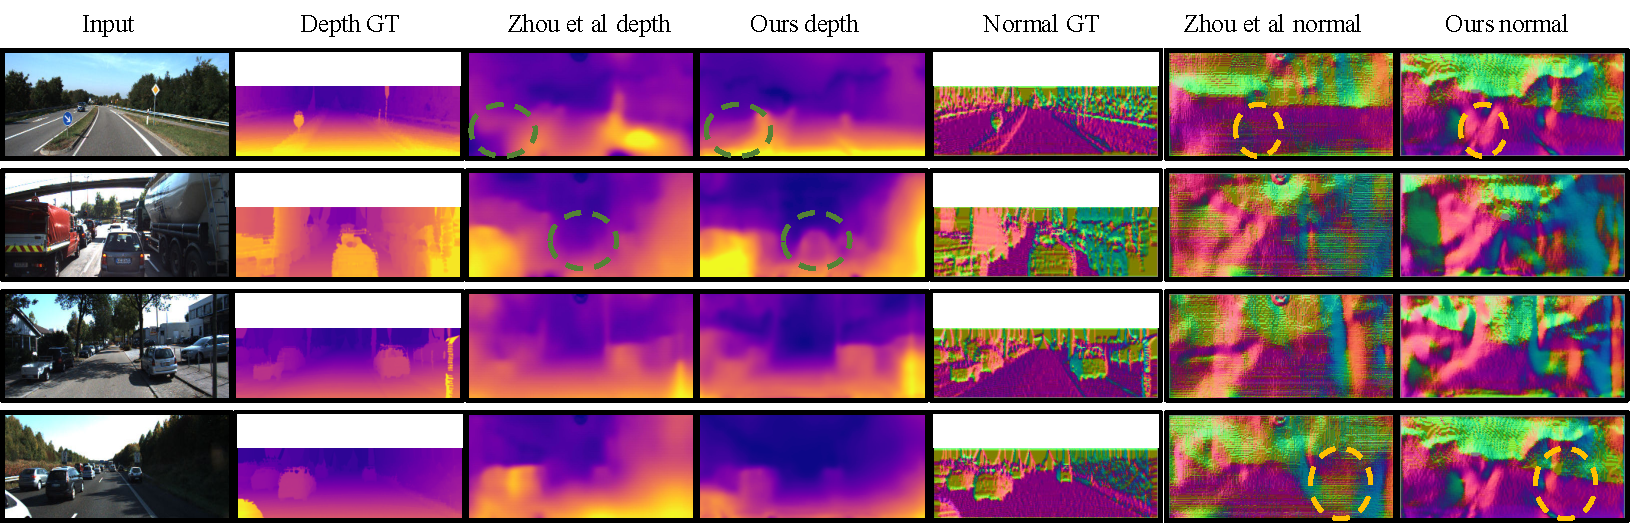
\includegraphics[width=\textwidth]{figures/examples_7col_comp.pdf}
%\caption{1}
\caption{Visual comparison of depth and normal results between \protect\cite{zhou2017unsupervised} and ours. As the original depth ground truth map comes from sparse laser measurement, the interpolated depth map is shown for better visualization. As can be seen from the depth estimation, our results preserve the small/thin structures which have similar color to other foregrounds (green circles). From the normal comparison, our results predict the road normal direction better and have no artifact. The edges in normal map are also preserved better in our results (yello circles).}
\vspace{-1.0\baselineskip}
\label{fig:examples}
\end{figure*}

\begin{figure}[h]
\centering
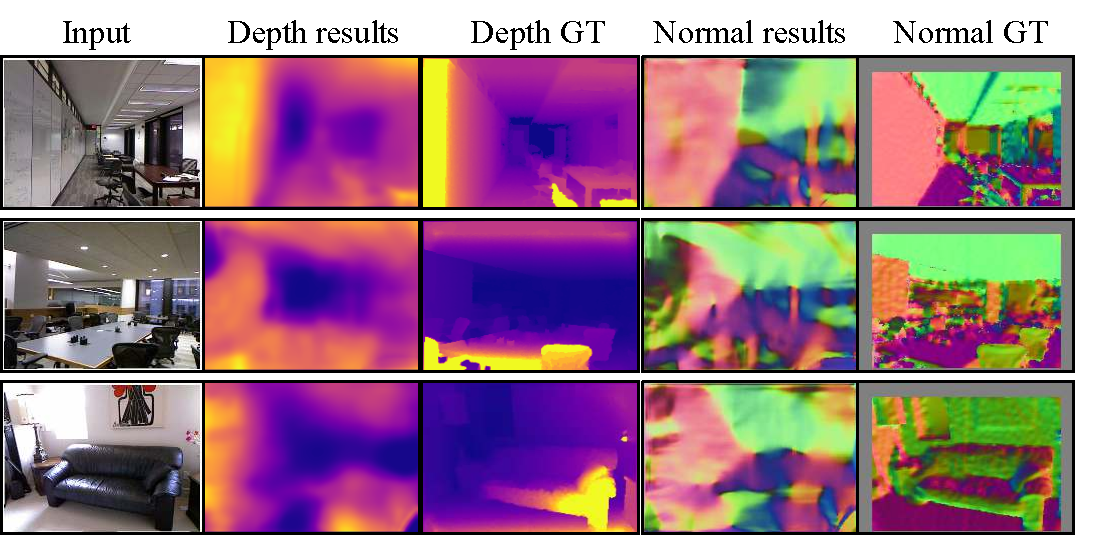
\includegraphics[width=0.5\textwidth]{figures/indoor_visual_comp.pdf}
\caption{Qualitative results of our framework on a subset of NYU v2 dataset.}
\vspace{-1.\baselineskip}
\label{fig:nyu_visual}
\end{figure}

To the best of our knowledge, there is no work reporting normal performance on the KITTI dataset. We thus compare the our normal predictions with that computed from the depth maps predicted by \cite{zhou2017unsupervised}. As shown in Tab. \ref{tbl:normal}, our method outperforms the baseline under all metrics. Additionally, to ensure the model is learned reasonably, we set up two naive baselines. ``Ground truth normal mean'' is that we set a mean normal direction for all pixels using ground truth normals. ``Pre-defined scene'' is that we separate the image to 4 parts using 4 lines connecting each image corder and image center. We set the bottom part having up-directed normal, left part having right-directed normal, right part having left-directed normal and top part with outward normals. Both of the baselines are significantly worse than our predicted model, demonstrating the correctness of the learned model.

%  and \cite{godard2016unsupervised}

% To our knowledge, there has not been works that report normal performance on KITTI 2015 dataset. We thus compare our normal performance with baseline methods and normals generated by applying depth-to-normal layer on depth maps of \cite{zhou2017unsupervised}. The baseline methods include ground truth normal mean, normals from pre-defined scene, our framework without second stage training, \ie without normal smoothness term and our full framework. As shown in Tab. \ref{tbl:normal}, our full model outperforms other methods under all metrics.

\begin{table}[t] \small
\centering
\caption{Normal performances of our method and some baseline methods.}
\label{tbl:normal}
\fontsize{6.5}{7}\selectfont
\bgroup
\def\arraystretch{1.2}
\begin{tabular}{l|c|c|c|c|c}
\thickhline
Method                        & Mean  & Median & $11.25^{\circ}$ & $22.5^{\circ}$  & $30^{\circ}$    \\ \hline
Ground truth normal mean      & 72.39 & 64.72  & 0.031 & 0.134 & 0.243 \\
Pre-defined scene             & 63.52 & 58.93  & 0.067 & 0.196 & 0.302 \\
\cite{zhou2017unsupervised} & 50.47 & 39.16  & 0.125 & 0.303 & 0.425 \\
Ours w/o normal smoothness    & 49.30 & 36.83  & 0.138 & 0.343 & 0.436 \\
Ours                          & 47.52 & 33.98  & 0.149 & 0.369 & 0.473 \\ \hline
\end{tabular}
\egroup
\vspace{-1.0\baselineskip}
\end{table}


\vspace{-0.7\baselineskip}
\paragraph{Indoor scene exploration.}
Besides the outdoor dataset, we also try to apply our framework on the indoor NYUv2 dataset \cite{silberman2012indoor}. We use a subset for some preliminary experiments. Specifically, ``study room" is picked and split for training and testing. We first try with our baseline method~\cite{zhou2017unsupervised}, and it fails to predict any reasonable depth maps. However, as shown in Fig. \ref{fig:nyu_visual}, our framework performs reasonably good on scenes that have multiple intersecting planes. Nevertheless, we still fail on scenes that have only a clutter of object. In the future, we plan to explore more on stronger feature matching rather than just using color matching, which may facilitate the learning under cluttered scenes.

